\documentclass[a4paper, 11pt]{article}
\usepackage[polish]{babel}
\usepackage[MeX]{polski}
\usepackage[utf8]{inputenc}
\usepackage[T1]{fontenc}
%\usepackage{times}
\usepackage{graphicx,wrapfig}
%\usepackage{anysize}
%\usepackage{tikz}
%\usetikzlibrary{calc,through,backgrounds,positioning}
\usepackage{anysize}
\usepackage{float}
%\usepackage{stmaryrd}
%\usepackage{amssymb}
%\usepackage{amsthm}
%\marginsize{3cm}{3cm}{3cm}{3cm}
%\usepackage{amsmath}
%\usepackage{color}
%\usepackage{listings}
%\usepackage{enumerate}
%\lstloadlanguages{Ada,C++}


\begin{document}	
	% \noindent -  w tym akapicie nie bedzie wciecia
	% \ indent - to jest aut., ale powoduje ze jest wciecie
	% \begin{flushleft}, flushright, center - wyrownianie akapitu
	% \textbf{pogrubiany tekst}
	% \textit{kursywa} 
	% 					STRONY 
	%  http://www.codecogs.com/latex/eqneditor.php 
	%  http://www.matematyka.pl/latex.htm
	% 
	\begin{titlepage}
		
		
		
		\newcommand{\HRule}{\rule{\linewidth}{0.5mm}} % Defines a new command for the horizontal lines, change thickness here
		
		\center % Center everything on the page
		
		%----------------------------------------------------------------------------------------
		%	HEADING SECTIONS
		%----------------------------------------------------------------------------------------
		
		\textsc{\LARGE Akademia Górniczo-Hutnicza im. Stanisława Staszica}\\[1.5cm] % Name of your university/college
		\textsc{\Large Kraków}\\[0.5cm] % Major heading such as course name
		\textsc{\large }\\[0.5cm] % Minor heading such as course title
		
		%----------------------------------------------------------------------------------------
		%	TITLE SECTION
		%----------------------------------------------------------------------------------------
		
		\HRule \\[0.4cm]
		{\fontsize{38}{50}\selectfont Symulator pożaru lasu}
		%	{ \Huge \bfseries} Symulator pożaru lasu\\[0.3cm] % Title of your document
		\HRule \\[1.5cm]
		
		%----------------------------------------------------------------------------------------
		%	AUTHOR SECTION
		%----------------------------------------------------------------------------------------
		
		% If you don't want a supervisor, uncomment the two lines below and remove the section above
		\Large \emph{Autorzy:}\\
		Marcin \textsc{Jędrzejczyk}\\ % Your name
		Sebastian \textsc{Katszer}\\ % Your name
		Katarzyna \textsc{Kosiak} \\[3cm]\ % Your name
		
		
		%----------------------------------------------------------------------------------------
		%	DATE SECTION
		%----------------------------------------------------------------------------------------
		
		{\large \today}\\[3cm] % Date, change the \today to a set date if you want to be precise
		
		%----------------------------------------------------------------------------------------
		%	LOGO SECTION
		%----------------------------------------------------------------------------------------
		
		%\includegraphics{Logo}\\[1cm] % Include a department/university logo - this will require the graphicx package
		
		%----------------------------------------------------------------------------------------
		
		\vfill % Fill the rest of the page with whitespace
		
	\end{titlepage}
	
	%SPIS TRESI
	%
	%
	%
	%
	%
	%
	%
	%
	%
	
	\tableofcontents
	\vfill
	\newpage
	%\pagebreak
	
	%SEKCJE
	%opis zagadnienia, temat, problem, dlaczego chcemy to rozwiązacyać metodą ewolucyjnę
	%jakie są metody rozwiącania problemu, przegląd literatury,
	%proponowane rozwiązania (spójność)
	%czym się inspierowałyśmy
	%
	%
	%
	
	%\setlength{\parskip}{1ex plus 0.5ex minus 0.2ex}
	
	\section{Wstęp}
	\indent
	
	Niniejszy dokument stanowi opis zagadnienia symulowania pożarów lasów wraz z prezentacją symulatora rozprzestrzeniania się pożaru lasu opartego na automatach komórkowych.
	
	\addcontentsline{toc}{section}{Cele modelowania pożaru}
	\section*{Cele modelowania pożaru}
	\indent
	
	Modelowanie pożaru polega na próbie odtworzenia zachowania się ognia i poznaniu jego parametrów w zadanej sytuacji - m.in. szybkości rozprzestrzeniania się, kierunku i ilości wydzielanego ciepła, estymację skutków pożaru. Na parametry te mają oczywiście wpływ ilość, rodzaj i dokładność dostarczonych danych wejściowch, z których najważniejszym jest rodzaj paliwa. \\
	\indent Istniejące modele paliwowe definiują zestawy cech roślinności mających wpływ na ich palność. Najbardziej znane modele pożaru korzystają z głównych systemów klasyfikacji modeli paliwowych takich jak dynamiczne modele Scotta i Burgana czy trzynaście ``oryginalnych'' modeli paliwowych Andersona i Albiniego, które opisują roślinność w czasie pory suchej, kiedy to stopień zagrożenia pożarowego jest najwyższy. Zwiększa to trafność i przydatność symulacji pożarów podczas organizacji akcji pożarowych.
	
	
	
	
	%	As Anderson states “Fuel models are simply tools to help the user realistically estimate fire behavior. The user must maintain a flexible frame of mind and an adaptive method of operating to totally utilize these aids".[2]
	%napisac o tym ze istnieje wiele modeli it te 13 oryginalnych ze w 
	% dry season bo po to sa symulacje, jakis cytat trzasnac.
	
	% wiki Fuel_model <- dużo info na temat paliw
	%	- fuel model dla naszego empirycznego, only for DRY SEASON!
	%	fala huygensa\\
	
	
	
	
	\addcontentsline{toc}{section}{Czynniki środowiskowe}
	\section*{Czynniki środowiskowe}%spradźcie czy to się trzyma kupy
	
	\indent 
	
	Na pożar lasu wpływ mają takie czynniki jak pogoda, charakterystyka paliwa i topografia terenu.	\\
	\indent
	Pogoda wpływa na ogień poprzez kierunek i siłę wiatru oraz wilgotność powietrza. Mokre paliwo potrzebuje więcej dostarczonej energii, by nastąpił jego zapłon. Ilość potrzebnej energii zależy również od temperatury otoczenia.	\\
	\indent
	Topologia ma znaczący wpływ na przebieg pożaru lasu. Jeżeli las jest na terenie pochyłym to ogień będzie rozprzestrzeniał się szybciej z dołu do góry niż odwrotnie, a to dzięki wstępnemu ogrzaniu drzew położonych wyżej. Dochodzi do tego jeszcze nasłonecznienie stoku. Jeśli drzewa są dobrze nasłonecznione oznacza to, że dostarczono im więcej energii, co przekłada się na ich szybszy zapłon niż drzew z zacienionego obszaru. Ukształtowanie terenu ma też wpływ na wiatr. Obecność gór, wąwozów oraz przełęczy zmienia przepływ powietrza.Ponadto mogą wystąpić bariery dla ognia takie jak drogi, uskoki w ziemi, rzeki, bagna, jeziora, które zatrzymują rozprzestrzenianie się ognia.\\
	\indent
	Wiatr działa na pożar na parę sposobów. Dostarcza tlen potrzebny podczas spalania. Zmniejsza wilgotność paliwa przez zwiększenie parowania. Także fizycznie przesuwa ogień i ciepło zwiększając zasięg pożaru. Co więcej jest odpowiedzialny za "spotting" (z ang.), czyli transport płonących kawałków drzew i niedopałków dalej w teren.\\
	\indent
	Paliwo pożaru to trawy, krzewy oraz wszystko inne co może się spalić. Drobne rzeczy zapalają się szybciej, a wielkie wolniej, ale też dostarczają różną ilość ciepła zależy - to od kaloryczności materiału, który płonie. Paliwo ma także wpływ na to w jaki sposób rozprzestrzenia się ogień. Dzięki wyższej roślinności możliwa wysokość słupa ognia naturalnie się zwiększa.  \\
	
	\addcontentsline{toc}{section}{Podejścia do modelowania pożaru}
	\section*{Podejścia do modelowania pożaru}
	\indent
	
	Od powstania pierwszych modeli pożarów w latach czterdziestych XX wieku minęło wiele czasu, w ciągu którego zaprezentowano kolejne - zróżnicowane pod względem wymaganych danych wejściowych, znaczących czynników i stopnia rozbudowania - modele.\\
	\indent	Problemem związanym z modelowaniem tak skomplikowanego zjawiska jak ogień jest rosnąca wraz z ilością branych pod uwagę czynników liczba koniecznych do wykoniania obliczeń, a co za tym idzie - potrzeba coraz większej mocy obliczeniowej. Właśnie  z powodu względnie długiego czasu symulacji i potrzeby dużej ilości danych wejściowych skomplikowane modele stosuje się częściej w badaniu niż w terenie.  W związku z tym w istniejących modelach zastosowano różne uproszczenia, często poświęcając mniej znaczące czynniki na rzecz przyspieszenia obliczeń.  \\
	\indent	Modele pożaru można podzielić na trzy grupy: empiryczne (model kanadyjski i australijski), semi-empiryczne (automaty komórkowe i Rothermel) i oparte na fizyce (modelowanie ognia koron oraz pełne fizyczne i multifazowe podejście).
	\subsection{Model paliwowy}	
	\indent
	
	Model paliwowy jest to zbiór możliwych paliw, typów roślinności i ich własności, które są reprezentowane w postaci parametrów. Parametry te wykorzystywane są następnie jako dane wejściowe dla zastosowanego modelu.\\
	
	Pierwszy taki zbiór wprowadził Rothermel, który rozróżnił 11 różnych paliw - od  krótkiej trawy po powalone drzewa - których właściwości utrzymują sie na stałym poziomie właściwości cząstek w czasie. Zbiór ten został rozszerzony o dwa modele paliw przez Albiniego, a następnie opisany przez Andersena. Wraz z czasem powstały bardziej rozbudowane zestawy. Narodziły się dynamiczne modele paliwowe. 
	
	\iffalse
	% \iftrue for disabling comment
	\subsubsection*{Modele empiryczne}
	\begin{itemize}
		\item Kanadyjski
		\item Australijski
	\end{itemize}
	\subsubsection*{Modele semi-empiryczne}
	\begin{itemize}
		\item Automaty komórkowe
		\item Rothermel
	\end{itemize}
	\subsubsection*{Modele oparte na fizyce}
	\begin{itemize}
		\item Modelowanie ognia koron 
		\item Pełne fizyczne i multifazowe podejście
	\end{itemize}
	\fi
	
	\addcontentsline{toc}{section}{Sztandarowe modele}
	\section* {Sztandarowe modele}
	\indent
	
	Poniżej znajduje się krótki przegląd kilku wartych uwagi modeli. Wszystkie wymienione miały znaczącą rolę w rozwoju zagadnienia modelowania pożaru lub są uznawane za najdokładniejsze dla zadanego czasu oczekiwania na rozwiązanie i używane są w najpopularniejszych profesjonalnych programach do symulacji pożaru jak na przykład Farasite, Prometheus czy BEHAVE, które dzięki swojej zdolności do oszacowywania zachowań ognia w czasie rzeczywistym demonstrują wielką użyteczność w terenie.
	\subsection{Rothermel - szybkość rozchodzenia się linii pożaru}
	\indent
	
	Pierwszy matematyczny model dla symulacji pożaru, został opublikowany w 1972 roku przez Richarda Rothermela.\\
	
	Przybliżone równanie na szybkość rozchodzenia się linii pożaru ma formę:
	$$
	R=\frac{(I_p)_{0}(1+\phi_W +\phi_S)}{\rho_b\epsilon Q_{ig}}\\
	$$
	%% to może kolega mi przetłumaczy lepiej niż google translator
	gdzie:\\
	$R$	- szybkość rozchodzenia się linii pożaru	[m/min]\\
	$(I_P)_0$	- 	strumień ciepła dla warunków bezwietrznych	[kJ/m2/min]\\
	$\rho_b$	- 	gęstość drewna całkowicie suchego	[kg/m3]\\
	$\epsilon$ 	- efektywność ogrzewania	\\
	$Q_{ig}$	- 	ciepło przed-zapłonowe	[kJ/kg]\\
	$\phi_w$	- 	współczynnik wiatru	\\
	$\phi_s$	- 	współczynnik nachylenia\\
	
	\subsubsection{Ciepło przed zapłonowe}	
	
	$Q_{ig}$	- 	ciepło przed-zapłonowe	[kJ/kg]\\
	Ciepło przed zapłonem jest to energia w przeliczeniu na jednostkę masy, która jest potrzebna do zapłonu. Obliczane jest na podstawie zmian ciepła właściwego z otoczenia, temperatury zapłonu, jak i ciepła utajonego wyparowywania wilgoci	.
	
	
	$$Q_{ig}=C_{pd}\Delta T_{ig} + M_{f}(C_{pw}\Delta T_{B}+V)$$
	gdzie:\\
	$C_{pd}$ - ciepło właściwe suchego drewna,\\
	$\Delta T_{ig}$ - zakres temperatur zapłonu,\\
	$M_{f}$ - wilgotność paliwa,\\
	$C_{pw}$ - ciepło właściwe wody,\\
	$\Delta T_{B}$ - Zakres temperatur wrzenia,\\
	$V$ - Utajone ciepło parowania.\\
	
	Po przeliczeniu:
	
	$$Q_{ig}=250+1,116M_{f}$$
	
	
	\subsubsection{Efektywność ogrzewania}
	
	Jest to stosunek efektywnej gęstości, czyli ilość paliwa, które bierze udział w zapłonie $p_{be}$, do rzeczywistej gęstości paliwa $p_{b}$
	$$\epsilon =  \frac{p_{be}}{p_{b}}$$
	
	Dana ta została wyliczona eksperymentalnie przez Rothermela i dla "dobrych paliw" przyjmuje wartość bliską jeden, a wraz ze wzrostem rozmiarów paliwa będzie maleć do $0$. 
	$$\epsilon=exp(-138/\sigma)$$ 
	gdzie:\\
	$\sigma$ - iloraz powierzchni i objętości cząsteczki paliwa. Dla paliw o kształcie walca współczynnik ten może przyjąć wartość:
	
	$$\epsilon=\frac{4}{d}$$ 
	gdzie:\\
	$d$ - Jest średnicą paliw okrągłych lub długością krawędzi przekroju kwadratowego.
	
	
	\subsubsection{Strumień ciepła}
	Czynnik $I_{p}$ określa, w jaki sposób rozchodzi się strumień ciepła. Składa się on z poziomego jak i pionowego strumienia. Istota wertykalnego strumienia pojawia się w momencie wiania wiatru, który to powoduje przechylenie się płomienia, powodując wzrost promieniowania podczerwonego. W modelu bezwietrznym pozostaje podstawowy, horyzontalny wektor $(I_{p})_{0}$, który to może zostać wyliczony eksperymentalnie w bezwietrznych warunkach.
	
	\subsubsection{Współczynnik wiatru, nachylenia}
	
	Współczynniki te reprezentują dodatkowe strumienie ciepła, które tworzone są przez dodatkowe warunki jakimi są siła wiatru i ukształtowanie terenu. Są to bezwymiarowe współczynniki, wyliczane w sposób eksperymentalny.
	
	\subsection{Rothermel - szybkość rozprzestrzeniania się pożaru w koronach}
	\indent
	
	Równanie opisujące szybkość rozprzestrzeniania się pożaru w koronach:
	$$
	R_{active}=3.34(R_10)_{40\%}
	$$
	gdzie: \\
	$R_{active}$ - szybkość rozprzestrzeniania się pożaru w koronach [m/min]\\
	$R_10$ - szybkość rozchodzenia się linii pożaru dla 10. modelu paliwowego i prędkość wiatru na wysokości połowy płomieni równa 40\% prędkości wiatru na wysokości 6,1m. [m/min]\\
	
	\subsection{Van Wagner - intensywność linii ognia}
	\indent
	Van Wagner zaproponował inne podejście do zagadnienia rozprzestrzenania się pożaru. Równanie opisujące intensywność linii ognia wymaganą do dalszego przeniesienia się ognia:
	$$
	I`_{initiation}=(\frac{CBH(460+25.9FMC)}{100})^{(\frac{3}{2})}
	$$
	gdzie:\\
	$I_initation$ - intensywność linii ognia wymaganą do dalszego przeniesienia się ognia [J/m] \\
	CBH - podstawowa wysokość roślinności [m]\\
	FMC- wilgotność roślinności (podłoża i drzew)\\
	%Pozwalam sobie wywalić na razie 
	\iffalse
	\subsection{Cruz(1999)}
	$$
	g(x)=\beta_0+\beta_{1}U_10+\beta_{2}FSG+ \sum\limits_{a=1}^{k_j -1}\beta_{ju}D_{ju}+\beta_5EFFM
	$$
	EFFM- estimated fine ful moisture content(\% ovendry mass basis)\\
	$U_10  10-m$ open wind speed
	$\beta_1, ...,\beta_4$ -regression coefficients
	\fi
	\subsection{Cruz - szybkość rozprzestrzeniania się pożaru w koronach}
	\indent
	Zaproponowane w 2002 roku przez Cruza równanie na szybkość rozprzestrzeniania się pożaru w koronach: 
	$$
	CROS_A=\beta_1U^{\beta_2}_10 \times CBD^{\beta_3} \times e^{-\beta_4EFFM}
	$$
	gdzie: \\
	$EFFM$ - estymowana wilgotność paliwa \\
	$CBD$ - gęstość grupy roślinności [1/m3]\\
	$U_10  10-m$ - prędkość wiatru ponad najwyższą roślinnością [m/min]\\
	$\beta_1, ...,\beta_4$ -współczynniki regresji\\
	\subsection{Modele oparte na automatach komórkowych}	
	\indent
	
	Automat komórkowy to system składający się z pojedynczych komórek, ktore znajdują sie jedna obok drugiej na n-wymiarowej siatce. Każda z komórek może mieć w danej chwili jeden stan z wielu. Stany komórki zmieniają się zgodnie z regułami przejść i zależą od stanu jej sąsiadów. Czas i przestrzeń są dyskretne.\\
	
	Automaty komórkowe tworzą środowisko dla większych dyskretnych klas modeli.
	\begin{figure}[H]
		\centerline{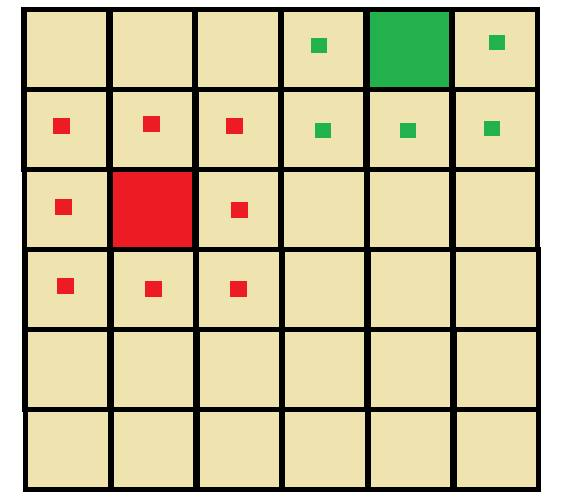
\includegraphics[scale=0.4]{automaty}}
		\raggedright{	\caption{Automaty komórkowe - przykładow prezentacji różnych stanów wraz z zaznaczonym sąsiedztwem Moore'a}}
	\end{figure}
	
	\section{Proponowany model}
	\indent
	
	Zastosowany w tej aplikacji model opiera się na modelu szybkości rozchodzenia się linii pożaru Rothermela, przy czym do reprezentacji lasu wykorzystana została sieć automatów komórkowych. Sąsiedztwo dla każdej komórki obliczane jest na podstawie wprowadzonych przez użytkownika danych i wykorzystuje zasadę Huygensa oraz opisaną poniżej zależność Andersona. \\
	
	\addcontentsline{toc}{section}{Cele modelu}
	\section*{Cele modelu}
	\indent
	
	Nasze cele to zapoznanie się z metodami przeprowadzania symulacji i próba przeniesienia wiedzy teoretycznej na projekt praktyczny. Ponadto celem jest przetestowanie jak radzi sobie język Java w tego typu projektach oraz ile z właściwości tego języka jesteśmy w stanie użyć przy tego rodzaju aplikacji.
	
	\addcontentsline{toc}{section}{Uzasadnienie wyboru danych narzędzi i technologii}
	\section*{Uzasadnienie wyboru danych narzędzi i technologii}
	\indent
	
	Nasz symulator został zaimplementowany w języku Java, ponieważ wszyscy członkowie zespołu są pragną rozwijać swoje zdolności programistyczne w tym języku, a także chcielibyśmy sprawdzić wydajność tego języka.\\
	
	Jeśli chodzi o bibliotekę graficzną, to nasz wybór padł na libGDX - crossplatformową bibliotekę z licencją opensource (oficjalna strona internetowa: www.libgdx.badlogicgames.com). \\
	
	Jedną z głównych zalet tej biblioteki jest jej szybkość - twórcy postawili bardzo duży nacisk na rozsądne zarządzanie pamięcią.  Dodatkowo libGDX dostarcza narzędzi do obsługi dźwięku i interpretacji wejścia dostarczonego przez użytkownika. Mimo, że renderowanie zachodzi przy użyciu OpenGL ES 2.0, to w większości przypadków nie trzeba znać szczegółów działania tego API, ponieważ biblioteka libGDX dostarcza wygodnych, wysokopoziomowych metod, dzięki którym sprawnie można uzyskać pożądane efekty - od wyświetlania dwuwymiarowych obiektów po tworzenie trójwymiarowych scen.\\
	
	Diagramy UML zostały stworzone w programie starUML - jest to lekki, darmowy program, który oferuje przyjazny interfejs użytkownika i wygodną hierarchizację elementów.
	
	
	\addcontentsline{toc}{section}{Dane wejściowe}
	\section*{Dane wejściowe}
	\indent
	
	\noindent\begin{minipage}{0.4\textwidth}% adapt widths of minipages to your needs
		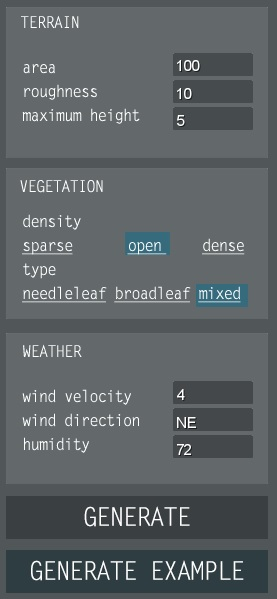
\includegraphics[width=\linewidth]{GUI}
		Interfejs użytkownika
	\end{minipage}%
	\hfill%
	\begin{minipage}{0.5\textwidth}\raggedright
		
		W celu uruchomienia symulacji na podstawie własnych danych należy podać:
		\begin{itemize}
			\item długość boku powierzchni (area),
			\item nierówność terenu (roughness),
			\item maksymalną wysokość terenu(maximum height),
			\item gęstość zalesienia (density),
			\item typ lasu (type),
			\item prędkość wiatru (wind velocity),
			\item kierunek wiatru (wind direction),
			\item wilgotność powietrza (humidity).
		\end{itemize}
		Aby wygenerować symulację na podstawie powyższych danych należy wcisnąć przycisk GENERATE.\\
		Przycisk GENERATE EXAMPLE jest odpowiedzialny za podstawienie danych testowych i wygenerowanie dla nich symulacji.
	\end{minipage}
	
	
	\addcontentsline{toc}{section}{Dane wyjściowe}
	\section*{Dane wyjściowe}
	\indent
	
	Wersja Beta, poza generowaniem symulacji, nigdzie nie zapisuje swoich wyników.
	
	\addcontentsline{toc}{section}{Sąsiedztwo}
	\section*{Sąsiedztwo}
	\indent	
	
	W naszym projekcie sąsiedztwo dla danego drzewa wyliczane jest na podstawie szybkości rozchodzenia się pożaru ze wzoru Rothermela, który to uwzględnia również współczynniki wiatru i nachylenia. Zastosowana została zasada Huygensa, która to zakłada, że każdy wierzchołek może być źródłem nowej eliptycznej ekspansji ognia. W związku z tym, sąsiedztwo komórki jest wygenerowane z elipsy. Jej kształt jest zgodny z zależnością odkrytą przez Andersona, przy założeniu, że pożar rośnie w kształcie pojedynczej elipsy, zgodnie z założeniami modelu Alexandra. Fizycznie tworzona jest ona w układzie współrzędnych biegunowych, gdzie zostaje obrócona wraz z kierunkiem wiania wiatru. Następnie jest ona rzutowana na rzeczywiste położenie komórki i poddana dyskretyzacji.
	\begin{figure}[H]
		\centerline{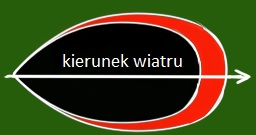
\includegraphics[scale=1.0]{elipse}}
		\raggedright{	\caption{Sąsiedztwo komórki generowane z elipsy}}
	\end{figure}
	
	
	%dsd
	%	Prędkość wiatru, ukształtowanie terenu. (może wgrywać mapę z wysokościami komórek
	%	i ona mogłąby być rozszerzana odpowiednio do rozmiaru!).
	\addcontentsline{toc}{section}{Modele paliwowe}
	\section*{Modele paliwowe}
	\indent	
	
	Nasza aplikacja pozwala użytkownikowi na wybranie jednego z trzech modeli paliwowych, które opisują najpowszechniejsze w Polsce typy lasów. Dodatkowo dla każdego z tych typów można zdefiniować gęstość lasu.
	Typ lasu:
	\begin{itemize}
		\item liściasty (broadleaf) - składający się w 85\% z dębów i w pozostałej części z sosen,
		\item iglasty (needleleaf) - składający się w 85\% z sosen i w pozostałej części z dębów,
		\item mieszany (mixed) - składający się z równej ilości sosen i dębów.
		
	\end{itemize}
	Gęstość lasu:
	\begin{itemize}
		\item las otwarty (open) - tylko 20\% terenu jest zajęte przez drzewa,
		\item las rzadki (sparse) - 50\% terenu jest zajęte przez drzewa,
		\item las gęsty (dense) - aż 80\% terenu jest zajęte przez drzewa,
		
	\end{itemize}
	
	%\addcontentsline{toc}{section}{$ f $ minmaxTransposition}
	\section*{Diagramy}
	\indent
	
	\begin{figure}[H]
		\centerline{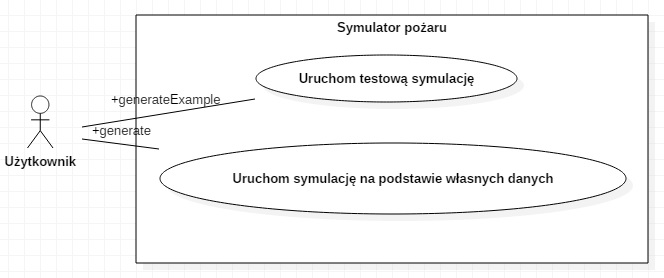
\includegraphics[scale=0.9]{usecase1}}
		\raggedright{	\caption{Diagram przypadków użycia}}
	\end{figure}
	
	\section{Wyniki symulacji}
	\indent
	W niniejszym rozdziale przedstawione zostaną wyniki testów naszej aplikacji.
	\addcontentsline{toc}{section}{Porównanie wyników z danymi rzeczywistymi}
	\section*{Porównanie wyników z danymi rzeczywistymi}
	\indent
	
	Do walidacji wykorzystaliśmy jako punkt odniesienia pożar Kuźni Raciborskiej w 1992 roku.
	Informacje z materiałów źródłowych o tym pożarze to m.in.:
	\begin{itemize}
		\item Klimat umiarkowany, kontynentalny z wpływem atlantyckiego,
		\item Średnia roczna opadów 650mm w części północnej, 660mm w części południowej, 500mm ostatniego lata,
		\item Udział drzew iglastych(sosna, świerk) w powierzchni- 85\%,
		\item Udział drzew liściastych(głównie dąb,buk, brzoza) w powierzchni- 15\%,
		\item Wiatr południowo-zachodni,
		%\item Prędkość wiatru od XX do YY, średnio  ZZ,
		\item Wiek drzew: do 20 lat - 15\%, do 40 lat 18\%, starsze 67\%,
		\item Teren nizinny, płaski, bez wyraźnych wzgórz czy znacznych różnic wysokości terenu,
		\item Temperatura w dniu pożaru wynosiła $34^\circ C$, a wcześniej nawet do 40$^\circ C$,
		\item Większość warstwy podłoża to niezmineralizowana ściółka lub zbutwiałe drzewa oraz rośliny o grubości kilkunastu cm,
		\item Obecność torfu o grubości 1-1.5m, który zajmował około 150ha obszaru.
	\end{itemize}
	<<<<<<< HEAD
	\section*{Pożar Kuźni Raciborskiej}
	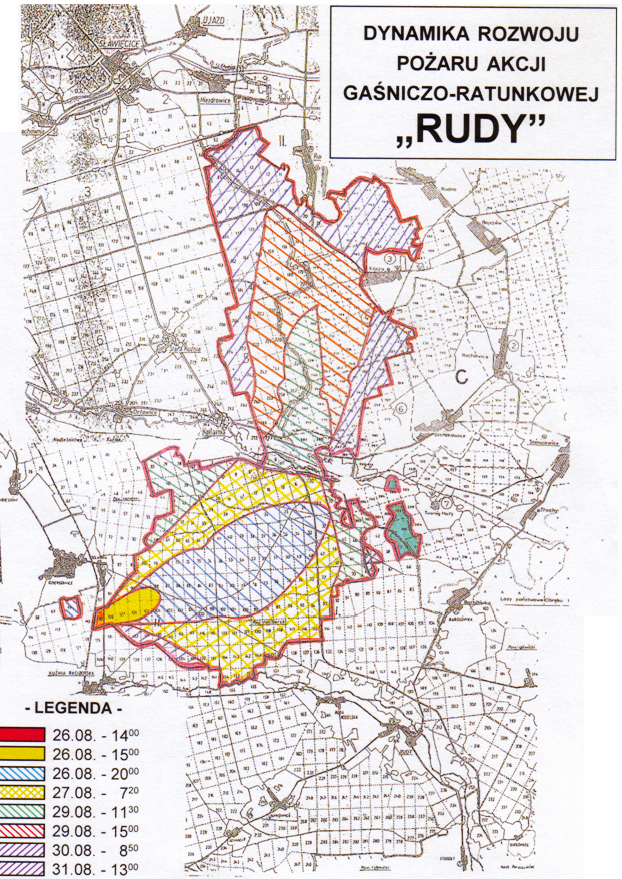
\includegraphics[scale=0.7]{kuzniaR.jpg}\\
	
	
	
	
	\section*{Wynik naszego programu dla danych o o Kuźni Raciborskiej}
	
	\begin{figure}[H]
		\centerline{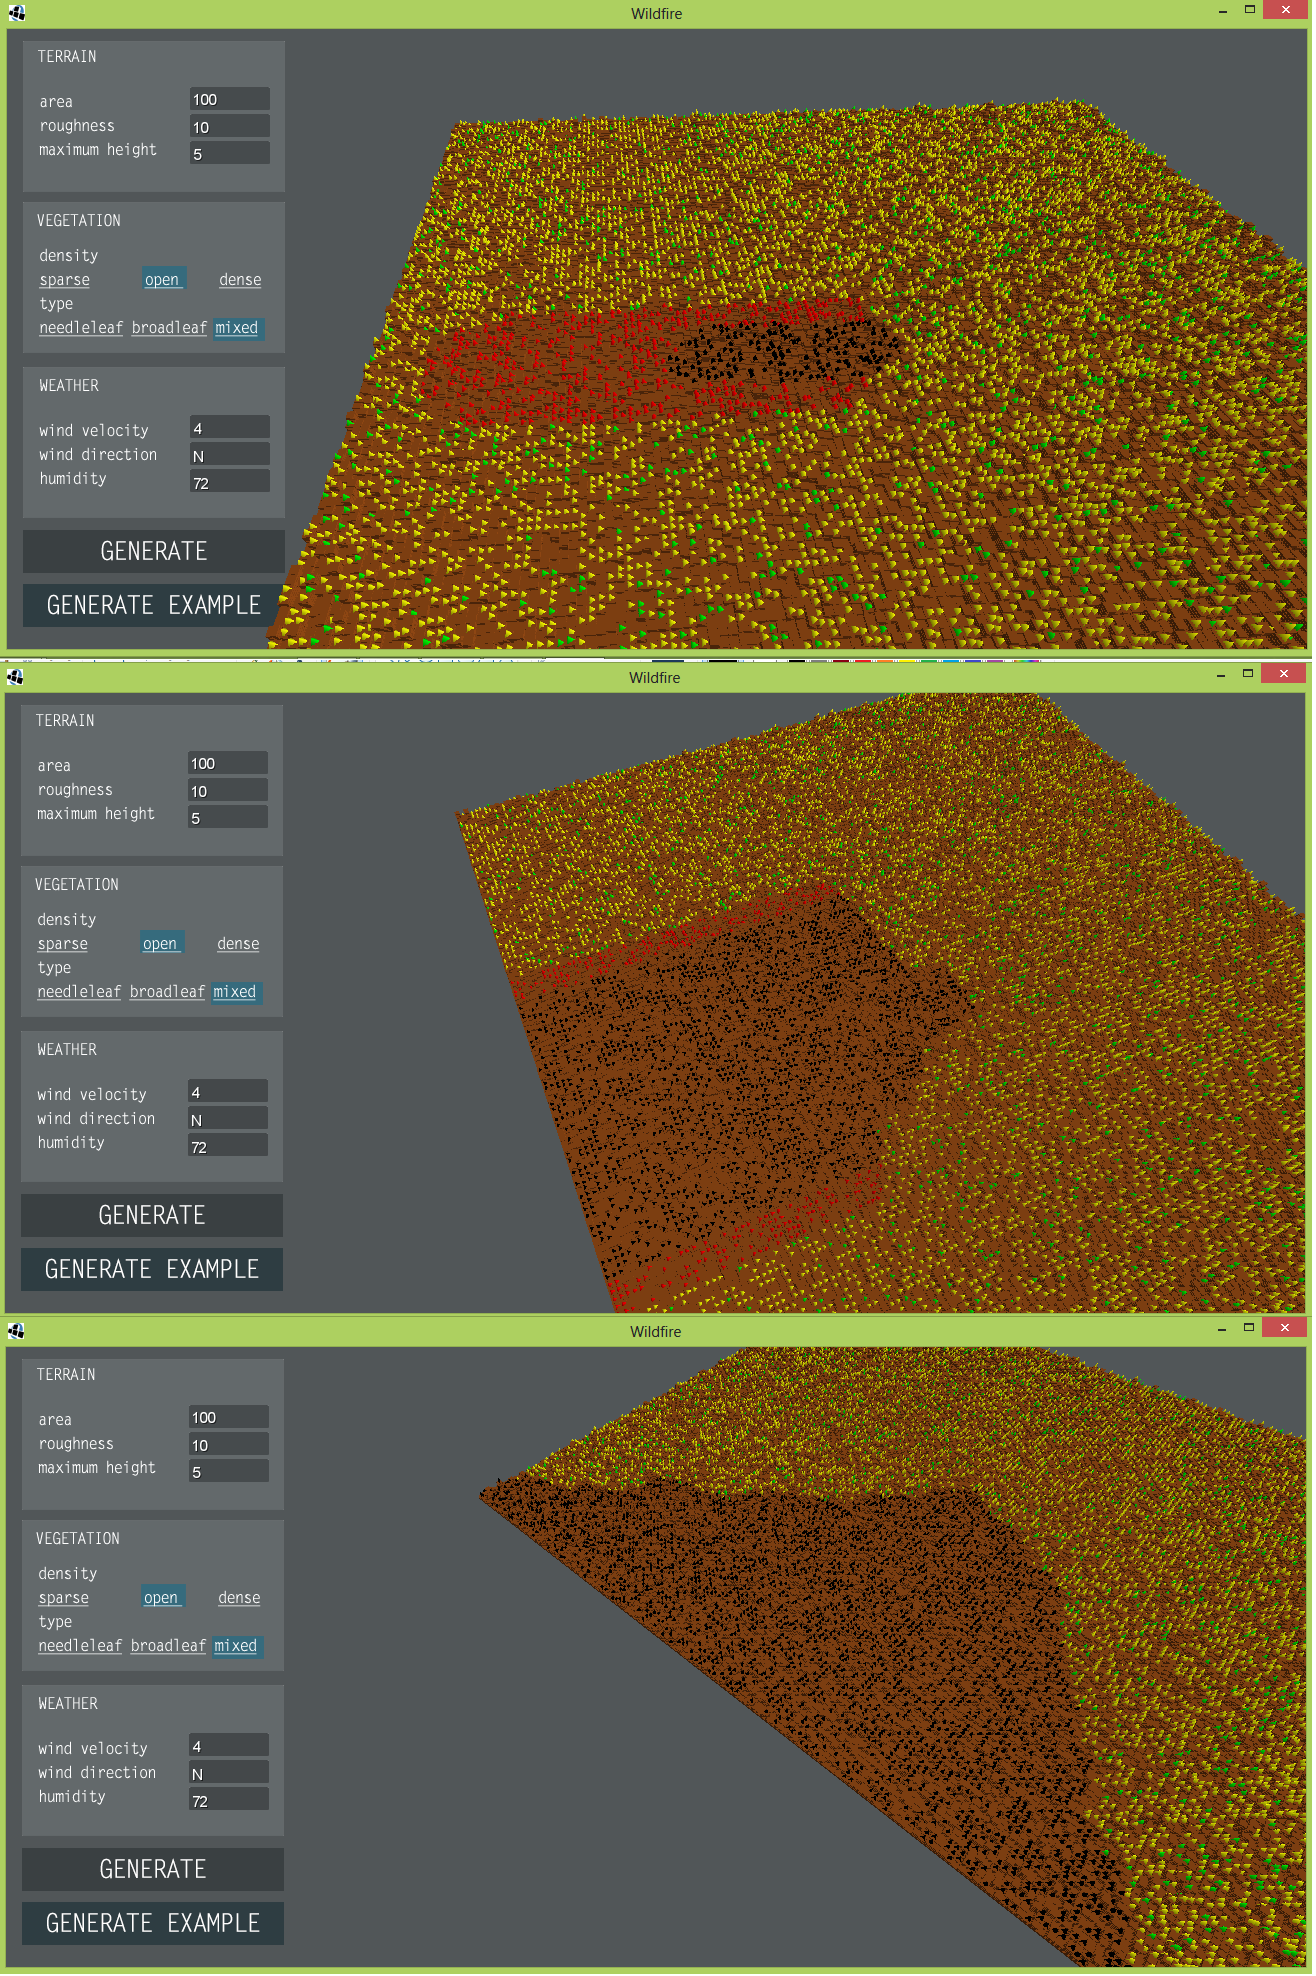
\includegraphics[scale=0.4]{kuzniatest}}
		\raggedright{	\caption{Wyniki naszej symulacji dla danych Kuźni Raciborskiej}}
	\end{figure}
	
	
	\section{Testy}
	\indent
	\begin{figure}[H]
		\centerline{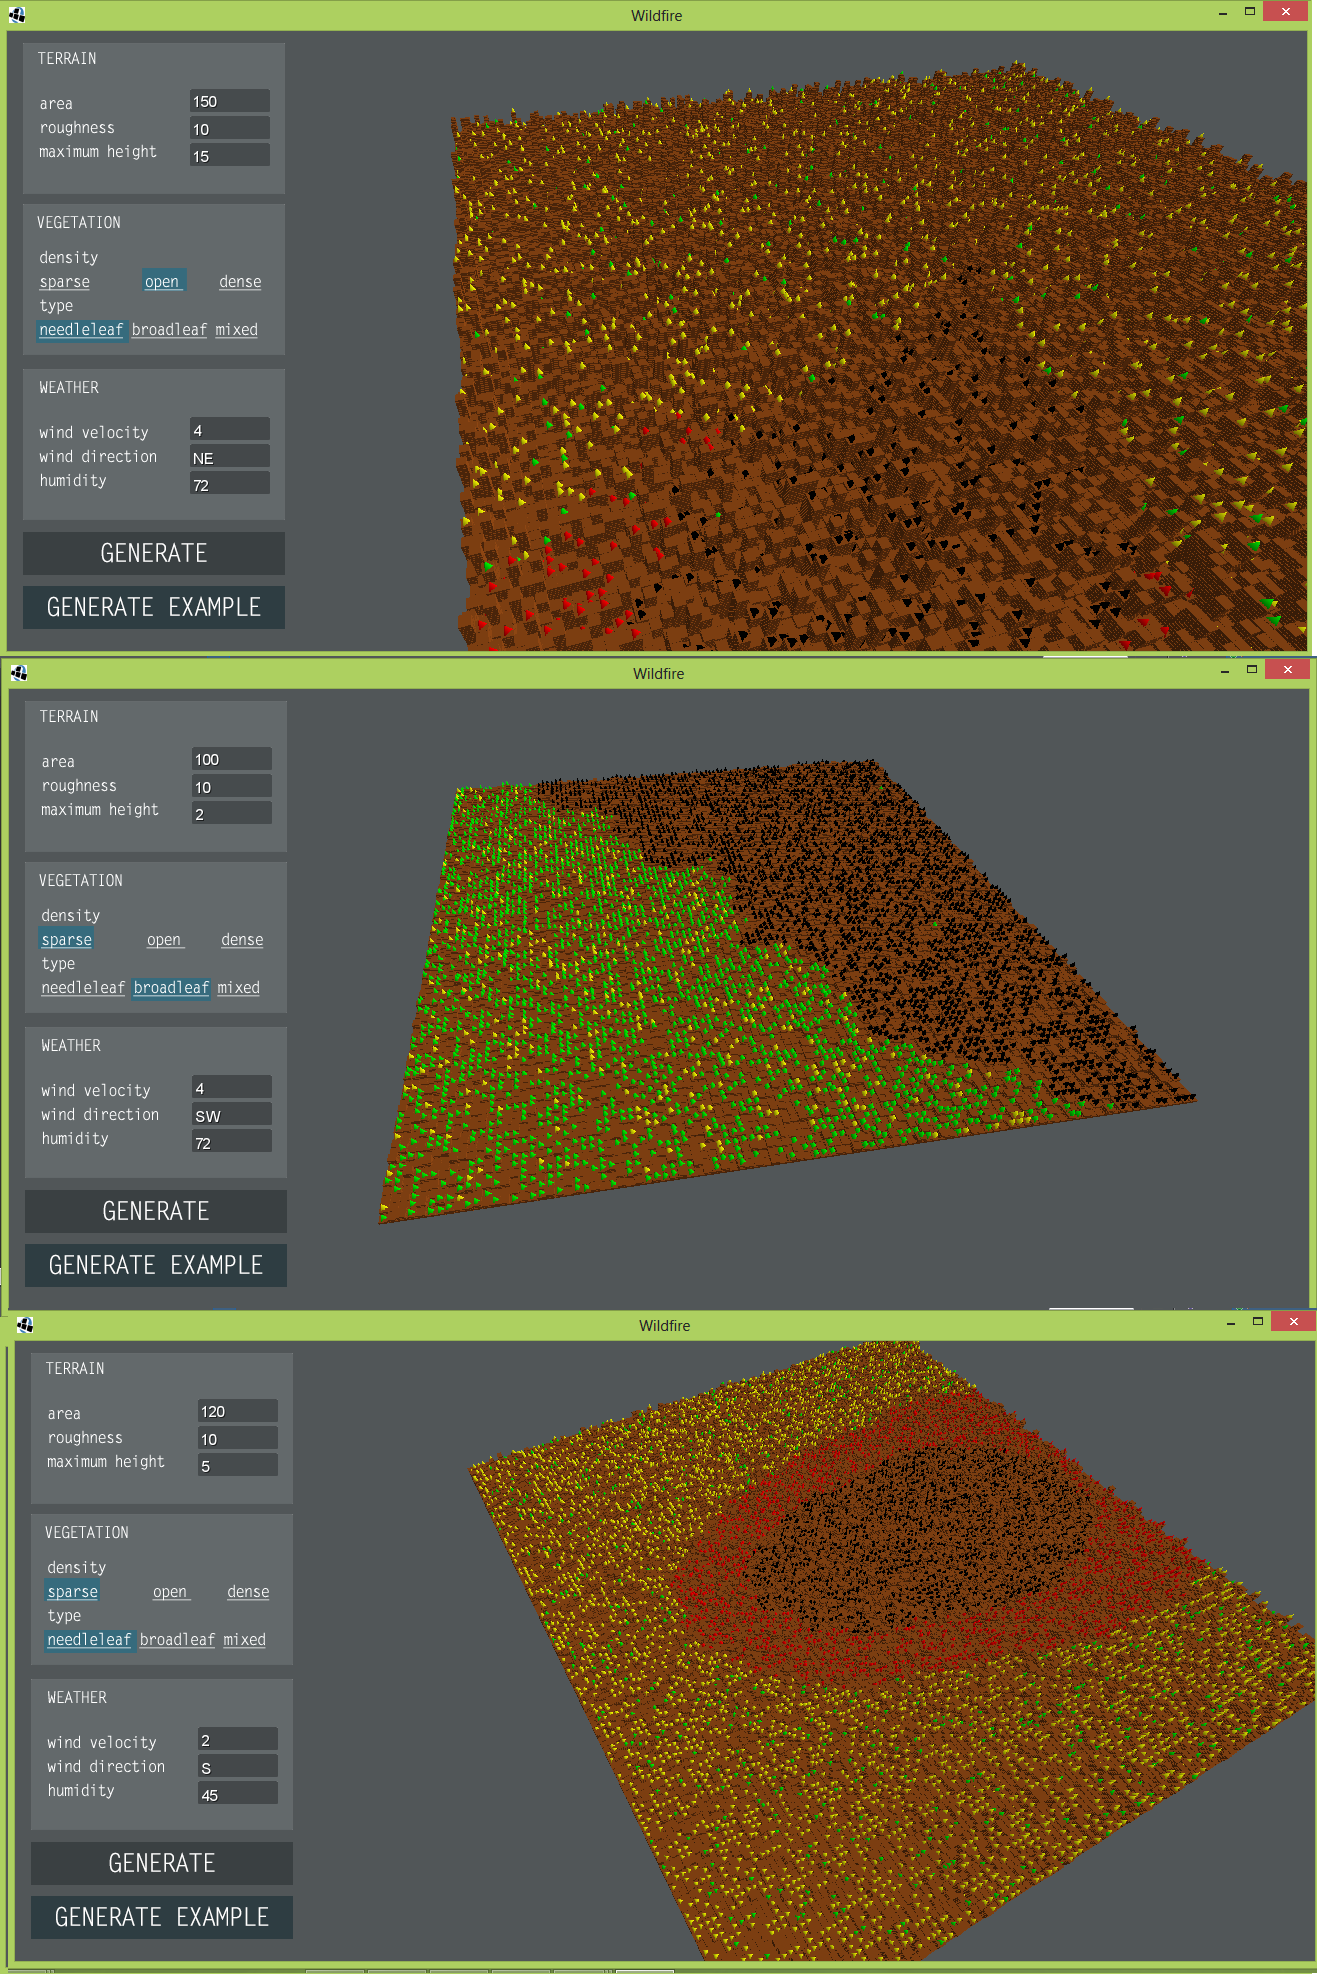
\includegraphics[scale=0.4]{generatetest}}
		\raggedright{	\caption{Przykładowe wyniki naszej symulacji dla danych wpisanych przez użytkownika}}
	\end{figure}
	
	\addcontentsline{toc}{section}{Statystyki}
	\section*{Statystyki}
	\indent
	sd
	\section{Wnioski}
	\indent
	
	sdsd
	\section{Literatura}
	%\indent
	
	\textbf{Asensio MI, Ferragut L., Simon J.:} Modelling of convective phenomena in forest fire. Rev Real Academia de Ciencias, 2002, 96:299–313\\
	\textbf{Bodrožić Ljiljana, Stipaniev Darko, Šerić Marijo:} Forest fires spread modeling using cellular automata approach, University of Split, 21000 Split, Croatia, 2009 \\
	\textbf{Chad Hoffman:} Fire Behavior Predictions Case Study, University of Idaho, 2007\\
	\textbf{Czerpak Tomasz, Maciak Tadeusz:} Modelowanie pożaru lasu. Część 1. Metody i algorytmy modelowania pożaru lasu, Wydział Informatyki, Politechnika Białostocka, 2011 \\
	\textbf{Kułakowski Krzysztof:} Automaty Komórkowe, OEN AGH (2000) \\
	\textbf{Law A.M., Kelton W.D.:} Simulation Modeling and Analysis, Second Edition, McGraw-Hill 2000\\
	\textbf{Ottmar Roger D. et al.:} "An Overview of the Fuel Characteristic Classification System - Quantifying, Classifying, and Creating Fuel beds for Resource Planning." Canadian Journal of Forestry Research. 37:2383-2393. 2007\\
	\textbf{Rothermel Richard C.:} A Mathematical Model for Predicting Fire Spread in Wildland Fuels. USDA Forest Service. Research Paper INT-115. 1972.\\
	\textbf{Sayama Hiroki:} Introduction to the Modeling and Analysis of Complex Systems, Open SUNY Textbooks, State University of New York at Geneseo, 2015\\	
	\textbf{Scott Joe H.,Burgan Robert E.:} Standard Fire Behavior Fuel Models, USDA Forest Service Gen. Tech. Rep. RMRS-GTR-153., June 2005\\	
	\textbf{Weise David R., Biging Gregory S.:} A Qualitative Comparison of Fire Spread Models Incorporating Wind and Slope Effects, Research Gate, October 2015\\
	\textbf{Wells Gail:} The Rothermel Fire-Spread Study: Still Running Like a Champ, Fire Science Direct, Issue 2, March 2008\\
	
	
	
	
	%to trzeba zrobić na podstawie zadania z latexa (9?) z odno
\end{document}
